\section*{Глава 2. Проектирование веб-приложения}
\addcontentsline{toc}{section}{Глава 2. Проектирование веб-приложения}
\stepcounter{section}

На данном этапе определяются роли пользователей и их права доступа, проектируются основные сценарии использования системы, формируется модель данных и описывается структура интерфейса. Результаты проектирования служат основой для последующей программной реализации системы.

\subsection{Определение ролей пользователей и прав доступа}

Для обеспечения безопасной и логичной работы системы необходимо заранее определить категории пользователей и круг доступных им действий. В проектируемом приложении используются три роли: администратор, преподаватель и студент.

Администратор обладает максимальным набором прав и отвечает за общее сопровождение системы. Он управляет учетными записями пользователей, ролями, категориями и всеми материалами, а также имеет доступ к просмотру статистики. Преподаватель работает с учебными материалами: создает их, редактирует собственные записи, прикрепляет файлы и при необходимости удаляет их. Студент использует приложение только как средство получения учебной информации, поэтому для него доступен просмотр материалов и скачивание файлов.

Матрица прав доступа представлена в таблице.

\begin{center}
\small\begin{tabularx}{0.96\textwidth}{>{\raggedright\arraybackslash}p{7.8cm} >{\centering\arraybackslash}p{1.6cm} >{\centering\arraybackslash}p{2.1cm} >{\centering\arraybackslash}p{2.0cm}}
\toprule
\textbf{Функция} & \textbf{Адм.} & \textbf{Препод.} & \textbf{Студ.} \\
\midrule
Вход в систему и выход из нее & + & + & + \\
Просмотр списка материалов & + & + & + \\
Просмотр карточки материала & + & + & + \\
Создание материалов & + & + & -- \\
Редактирование собственных материалов & + & + & -- \\
Удаление материалов & + & + & -- \\
Загрузка файлов к материалам & + & + & -- \\
Удаление файлов из материалов & + & + & -- \\
Просмотр категорий & + & + & -- \\
Управление категориями & + & -- & -- \\
Управление пользователями & + & -- & -- \\
Просмотр статистики & + & -- & -- \\
\bottomrule
\end{tabularx}
\end{center}

Выбранное распределение прав позволяет сохранить необходимый уровень безопасности и при этом не усложняет взаимодействие пользователей с системой.

\subsection{Проектирование функциональности приложения и сценариев использования}

Проектируемое приложение должно обеспечивать базовый набор пользовательских сценариев, связанных с управлением учебными материалами. На этапе проектирования были выделены основные функции системы: вход пользователя в систему, управление учетными записями, управление категориями, работа с материалами и файлами, а также просмотр статистики.

Основные пользовательские сценарии можно описать следующим образом:

\begin{itemize}[leftmargin=1.25cm]
    \item администратор входит в систему, создает пользователей, назначает им роли, управляет категориями и контролирует наполнение архива;
    \item преподаватель входит в систему, создает новый материал, заполняет его описание, выбирает категорию и прикрепляет файлы;
    \item преподаватель при необходимости редактирует собственный материал, обновляет информацию и удаляет ненужные файлы;
    \item студент входит в систему, просматривает список материалов, открывает карточку нужного материала и скачивает прикрепленный файл;
    \item администратор открывает страницу статистики и анализирует распределение материалов по категориям, авторам и ролям пользователей.
\end{itemize}

Для наглядного представления взаимодействия пользователей с системой в проект была включена диаграмма вариантов использования. На диаграмме отражены основные акторы системы --- администратор, преподаватель и студент --- и показаны ключевые действия, которые доступны каждой роли.

\begin{figure}[h!]
    \centering
    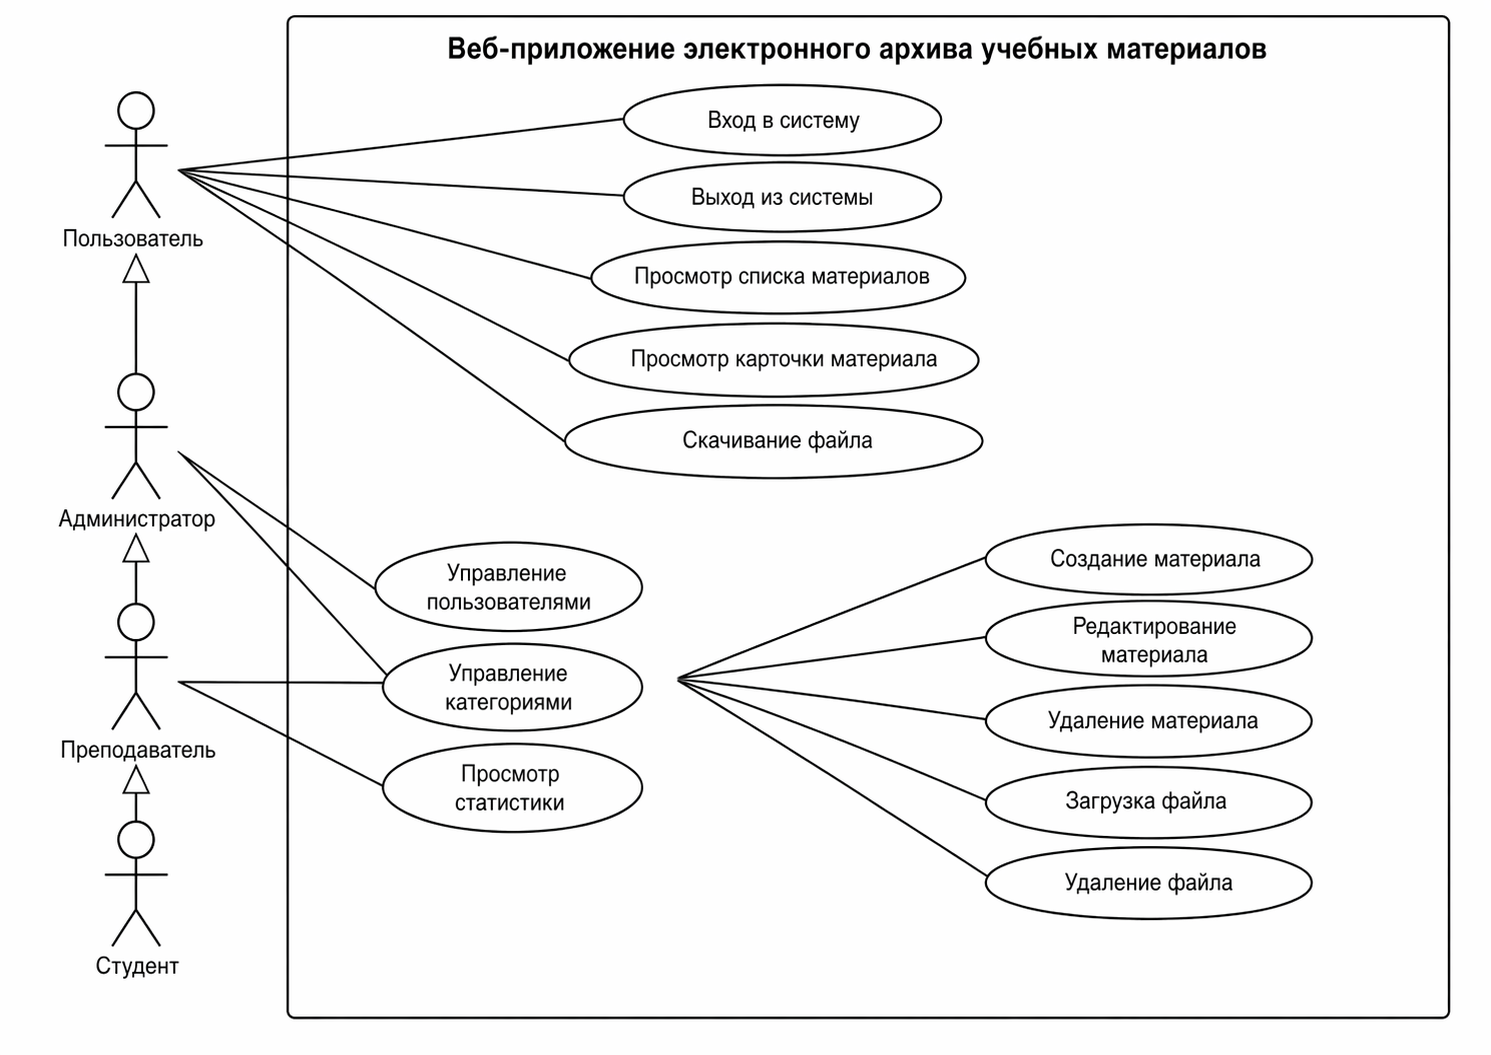
\includegraphics[width=0.92\textwidth]{images/use_case_diagram.png}
    \caption{Диаграмма вариантов использования веб-приложения}
\end{figure}

Диаграмма вариантов использования подтверждает, что проектируемая система охватывает все основные пользовательские сценарии, предусмотренные заданием: аутентификацию, разграничение прав доступа, работу с материалами и файлами, а также просмотр статистики администратором.

Для удобства навигации проектируется следующий состав страниц приложения:

\begin{longtable}{>{\raggedright\arraybackslash}p{4.2cm} >{\raggedright\arraybackslash}p{9.8cm}}
\toprule
\textbf{Страница} & \textbf{Назначение} \\
\midrule
\endfirsthead

\toprule
\textbf{Страница} & \textbf{Назначение} \\
\midrule
\endhead

\bottomrule
\endlastfoot

Главная страница & Краткая информация о системе и переход к основным разделам \\
Страница входа & Ввод логина и пароля пользователя \\
Список пользователей & Просмотр и управление учетными записями \\
Список категорий & Просмотр и администрирование категорий материалов \\
Список материалов & Просмотр всех материалов с возможностью фильтрации \\
Карточка материала & Просмотр описания материала и прикрепленных файлов \\
Страница создания и редактирования материала & Ввод названия, описания, категории и загрузка файлов \\
Страница статистики & Отображение агрегированных сведений по материалам, файлам и пользователям \\
\end{longtable}

Спроектированная функциональность приложения соответствует поставленной цели и позволяет реализовать все обязательные элементы курсового проекта.

\subsection{Проектирование модели данных для сущностей}

На этапе проектирования модели данных были выделены основные сущности предметной области: \texttt{Role}, \texttt{User}, \texttt{Category}, \texttt{Material} и \texttt{StoredFile}. Каждая из них отражает отдельный аспект работы системы.

Сущность \texttt{Role} используется для хранения названия роли и ее описания. Сущность \texttt{User} содержит данные пользователя: логин, хэш пароля, ФИО, дату создания учетной записи и ссылку на роль. Сущность \texttt{Category} предназначена для систематизации учебных материалов. Сущность \texttt{Material} хранит сведения о самом материале: название, описание, дату создания, автора и категорию. Сущность \texttt{StoredFile} содержит информацию о прикрепленных файлах: оригинальное имя, внутреннее имя хранения, путь к файлу и дату загрузки.

Связи между сущностями можно описать следующим образом:

\begin{itemize}[leftmargin=1.25cm]
    \item одной роли соответствует множество пользователей;
    \item одному пользователю может соответствовать множество материалов;
    \item одной категории может соответствовать множество материалов;
    \item одному материалу может соответствовать множество прикрепленных файлов.
\end{itemize}

Проектируемая модель данных представлена в таблице.

\begin{center}
\begin{tabularx}{0.96\textwidth}{>{\raggedright\arraybackslash}p{2.9cm} >{\raggedright\arraybackslash}p{4.8cm} >{\raggedright\arraybackslash}X}
\toprule
\textbf{Сущность} & \textbf{Основные атрибуты} & \textbf{Назначение} \\
\midrule
Role & id, name, description & Хранение ролей пользователей \\
User & id, username, password\_hash, full\_name, created\_at, role\_id & Хранение учетных записей пользователей \\
Category & id, name, description & Классификация учебных материалов \\
Material & id, title, description, created\_at, author\_id, category\_id & Описание учебного материала \\
StoredFile & id, original\_name, stored\_name, file\_path, uploaded\_at, material\_id & Хранение информации о прикрепленных файлах \\
\bottomrule
\end{tabularx}
\end{center}

Такая модель данных достаточно проста для реализации, но при этом полностью покрывает все требования.

\subsection{Проектирование структуры интерфейса и макетов основных страниц}

На этапе проектирования интерфейса была принята цель сделать приложение максимально простым и понятным. Пользователь должен быстро переходить между основными разделами системы и выполнять типовые операции без лишних действий.

В основе интерфейса лежит единый базовый шаблон страницы, содержащий верхнее меню навигации, название системы, ссылки на доступные разделы и область отображения системных сообщений. Такое решение обеспечивает единый внешний вид всех страниц приложения.

Для основных страниц были определены следующие элементы интерфейса:

\begin{itemize}[leftmargin=1.25cm]
    \item для страницы входа --- форма авторизации с полями логина и пароля;
    \item для страницы пользователей --- таблица со списком учетных записей и кнопками создания, редактирования и удаления;
    \item для страницы категорий --- таблица категорий и форма их добавления или изменения;
    \item для страницы материалов --- таблица или карточки материалов, фильтр по категории и ссылки на просмотр и редактирование;
    \item для карточки материала --- название, описание, сведения об авторе, категория, список прикрепленных файлов и кнопки действий;
    \item для страницы статистики --- набор таблиц с агрегированными данными по материалам, файлам, категориям и пользователям.
\end{itemize}

Проектируемая структура интерфейса позволяет легко масштабировать приложение и при необходимости дополнять его новыми разделами. При этом выбранный подход не перегружает пользователя и соответствует учебному характеру проекта.